\documentclass[12pt]{article}
\usepackage[margin=0.8in]{geometry}
\usepackage[utf8]{inputenc}
\usepackage{graphicx}
\usepackage[export]{adjustbox}
\graphicspath{ {../Images/} }
\usepackage{amsmath}
\usepackage{amsfonts}
\usepackage{amssymb}
\usepackage[version=4]{mhchem}
\usepackage{stmaryrd}
\usepackage{bbold}
%\usepackage[fallback]{xeCJK}
\usepackage{polyglossia}
\usepackage{fontspec}
%\setCJKmainfont{Noto Serif CJK TC}

\usepackage{tikz}
\usepackage{amsthm}
\usepackage{tcolorbox}
\usepackage{enumitem}% http://ctan.org/pkg/enumitem

\tcbuselibrary{theorems}

\definecolor{GrayBG}{HTML}{d9d9d9}
\definecolor{BlueDef}{HTML}{104e8b}
\definecolor{GreenProp}{HTML}{025540}
\definecolor{RedMet}{HTML}{cd5556}
\definecolor{BrownHist}{HTML}{8b5a2b}
\definecolor{BlackSav}{HTML}{000000}

\newcommand{\hideM}[1]{\mbox{\vphantom{$#1$}\smash{\colorbox{gray!50}{$\displaystyle #1$}}} }
\newcommand{\hide}[1]{\mbox{\vphantom{#1}\smash{\colorbox{gray!50}{#1}}}}
%\newcommand{\hideM}[1]{\mbox{\vphantom{$#1$}\smash{\colorbox{gray!50}{\phantom{$\displaystyle #1$}}}} }
%\newcommand{\hide}[1]{\mbox{\vphantom{#1}\smash{\colorbox{gray!50}{\phantom{#1}}}}}

\newtcbtheorem
  []% init options
  {definition}% name
  {Définition}% title
  {%
    colback=GrayBG,
    colframe=BlueDef,
    fonttitle=\bfseries,
  }% options
  {def}% prefix

\newtcbtheorem
  []% init options
  {proposition}% name
  {Proposition}% title
  {%
    colback=GrayBG,
    colframe=GreenProp,
    fonttitle=\bfseries,
  }% options
  {prop}% prefix

\newtcbtheorem
  []% init options
  {method}% name
  {Méthode}% title
  {%
    theorem name,
    colback=GrayBG,
    colframe=RedMet,
    fonttitle=\bfseries,
  }% options
  {met}% prefix
  
\newtcbtheorem
  []% init options
  {history}% name
  {Histoire}% title
  {%
    theorem name,
    colback=GrayBG,
    colframe=BrownHist,
    fonttitle=\bfseries,
  }% options
  {hist}% prefix
  
\newtcbtheorem
  []% init options
  {savoir}% name
  {Savoir-faire du chapitre}% title
  {%
    theorem name,
    colback=GrayBG,
    colframe=BlackSav,
    fonttitle=\bfseries,
  }% options
  {sav}% prefix

\newtheoremstyle{break}
  {}
  {}
  {}
  {}
  {\bfseries}
  {}
  {\newline}
  {}
\theoremstyle{break}
\newtheorem*{example}{Exemple.}
\newtheorem*{examples}{Exemples.}
\newtheorem*{remark}{Remarque.}

\newenvironment{demo}[1][\proofname]{%
  \begin{proof}[#1]$ $\newline
}{%
  \end{proof}
}

\setmainlanguage{french}
%\setmainf[tikznode]ont{CMU Serif}

\title{
\vspace{4em}
\centering
\tcbset{colframe=BlackSav,colback=GrayBG}
\tcbox[tikznode]{
Chapitre 6 \\ Nombres premiers
}
}

\author{}
\date{}

\setlength\parindent{0pt}

\begin{document}
\maketitle

\tableofcontents

\newpage


\section{L'ensemble des nombres premiers}
\begin{definition}{}{}
Un entier naturel est un nombre premier s'il admet exactement deux diviseurs positifs : 1 et lui même.
\end{definition}

\begin{examples}
La liste des nombres premiers inférieurs à 30 est la suivante : $2 ; 3 ; 5 ; 7 ; 11 ; 13 ; 17 ; 19$; $23 ; 29$.
\end{examples}

\begin{remark}
L'entier 1 n'est pas un nombre premier car il n'admet qu'un seul diviseur.
\end{remark}

\begin{proposition}{}{}
Tout entier naturel supérieur ou égal à 2 est divisible par un nombre premier.
\end{proposition}

\begin{demo}
On va montrer par récurrence que la propriété $\mathcal{P}(n)$ :« Tout entier naturel compris entre 2 et $n$ est divisible par un nombre premier » est vraie pour tout entier $n \geqslant 2$.\\
Initialisation : Pour $n=2$, la propriété est vraie car 2 est divisible par 2 qui est premier.\\
Hérédité : Supposons que $\mathcal{P}(n)$ soit vraie pour un certain entier $n \geqslant 2$ et montrons qu'alors $\mathcal{P}(n+1)$ est vraie.\\
Soit $k$ un entier tel que $2 \leqslant k \leqslant n+1$. L'objectif est de montrer que $k$ est divisible par un nombre premier.\\
Si $2 \leqslant k \leqslant n$, d'après $\mathcal{P}(n)$, il est clair que $k$ est divisible par un nombre premier.\\
Si $k=n+1$, on distingue deux cas :

\begin{itemize}[noitemsep,topsep=0pt]
  \item Si $k$ est premier, il est divisible par lui-même donc par un nombre premier.
  \item Si $k$ n'est pas premier, cela signifie qu'il existe des entiers $a$ et $b$ tels que $k=a b$ et tels que $2 \leqslant a \leqslant n$ et $2 \leqslant b \leqslant n$.\\
On peut alors appliquer l'hypothèse $\mathcal{P}(n)$ à l'entier $a$. Ainsi, $a$ est divisible par un nombre premier $p$. Par conséquent, $p \mid a$ et $a \mid k$ donc, par transitivité, $p \mid k$.\\
Dans tous les cas, on a montré que $\mathcal{P}(n+1)$ est vraie.
\end{itemize}
\end{demo}

\begin{remark}
  La propriété de récurrence est ici un peu particulière. Elle concerne tout entier inférieur ou égal à $n$ et pas seulement l'entier $n$. On dit qu'il s'agit d'une propriété de récurrence forte.
\end{remark}

\begin{proposition}{}{}
Soit $n \geqslant 2$.
\begin{itemize}[noitemsep,topsep=0pt]
  \item Soit $n$ est un nombre premier;
  \item Soit $n$ est divisible par un nombre premier compris entre 2 et $\sqrt{n}$.
\end{itemize}
\end{proposition}

\begin{demo}
Soit $n \geqslant 2$. Supposons que $n$ ne soit pas premier.

Cela signifie qu'il existe des entiers $a$ et $b$, avec $a>1$ et $b>1$ tels que $n=a b$.
L'un des deux entiers $a$, ou $b$ est inférieur ou égal à $\sqrt{n}$ car sinon, on aurait $a b>n$.\\
Supposons par exemple, que $a \leqslant \sqrt{n}$ (le cas $b \leqslant \sqrt{n}$ se traite de la même manière).\\
D'après la propriété $1, a$ est divisible par un nombre premier $p$. Comme $p \mid a$ et $a \mid n$, on en déduit, par transitivité que $p \mid n$. De plus, on a bien $p \leqslant \sqrt{n}$.
\end{demo}

\begin{method}{Démontrer qu'un entier est premier}{}
\begin{itemize}[noitemsep,topsep=0pt]
  \item Dresser la liste de tous les nombres premiers inférieurs ou égaux à $\sqrt{n}$.
  \item Vérifier qu'aucun de ces nombres ne divise $n$.
\end{itemize}
\end{method}

\begin{example}
Montrer que l'entier 71 est premier.

~\\Solution :\\
Supposons par l'absurde que 71 ne soit pas premier.\\
Il existerait alors un diviseur premier de 71 compris entre 2 et $\sqrt{71}$.\\
Or $\sqrt{71}<9$. Ainsi, 71 serait divisible par l'un des entiers suivants : $2,3,5,7$.
\end{example}

\begin{itemize}[noitemsep,topsep=0pt]
  \item D'après les critères de divisibilité, il est clair que 2,3 et 5 ne divisent pas 71 .
  \item De plus, 7 ne divise pas 71 car le reste de la division de 71 par 7 est 1 .
\end{itemize}

Finalement, aucun de ces nombres ne divise 71, ce qui est absurde.\\
Cela signifie que 71 est premier.

\begin{proposition}{}{}
Il existe une infinité de nombres premiers.
\end{proposition}

\begin{demo}
Supposons par l'absurde qu'il n'existe qu'un nombre fini de nombre premiers.\\
On note $p_{1}, p_{2}, \ldots, p_{n}$ ces nombres premiers. On considère alors l'entier $N=p_{1} \times p_{2} \times \ldots \times p_{n}+1$.\\
D'après la propriété $1, N$ est divisible par l'un des nombres premiers.\\
Autrement dit, il existe $1 \leqslant i \leqslant n$ tel que $p_{i}$ divise $N$.\\
On a donc $N \equiv 0\left[p_{i}\right]$\\
Or, $N \equiv p_{1} \times p_{2} \times \ldots \times p_{n}+1 \equiv 1\left[p_{i}\right]$, ce qui est absurde.
\end{demo}


\noindent
\begin{minipage}{.7\textwidth}
  \begin{history}{Infinité des nombres premiers}{}
    L'infinité de l'ensemble des nombres premiers est énoncé et démontré dans les Éléments d'Euclide. Plus tard, les mathématiciens continuèrent d'étudier la répartition des nombres premiers. Par exemple, en utilisant les congruences, l'allemand Gustav Lejeune Dirichlet (1805-1859) a pu établir le théorème de progression arithmétique : si $a$ et $b$ sont premiers entre eux, il existe une infinité de nombres premiers de la forme $a n+b$.
  \end{history}
\end{minipage}
\hspace{1em}
\begin{minipage}{0.35\textwidth}
  \begin{tcolorbox}[colback=white,colframe=BrownHist]
    \centering
    %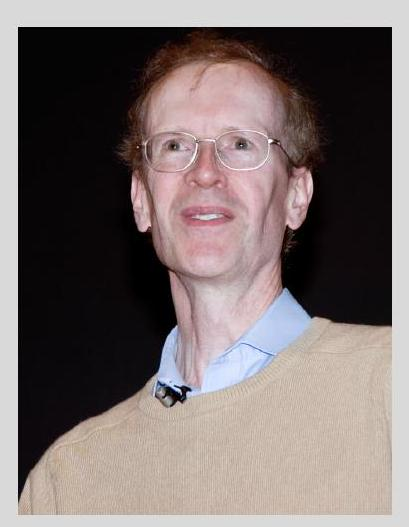
\includegraphics[max width=\textwidth, center]{2025_02_06_9ce8241190b3f203dae3g-7(1)}
    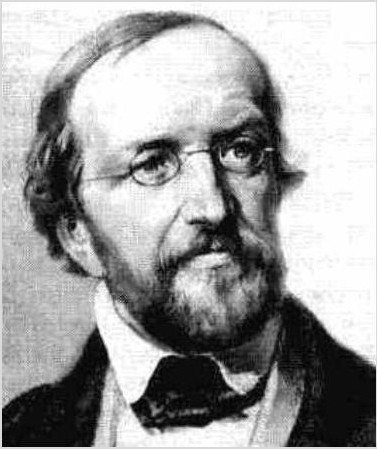
\includegraphics[max width=\textwidth, center]{2025_02_06_9ce8241190b3f203dae3g-3}
    Dirichlet
    %Andrew Wiles
  \end{tcolorbox}
\end{minipage}

\section{Décomposition en produit de facteurs premiers}
\begin{proposition}{}{}
Pour tout entier $n \geqslant 2$, il existe des nombres premiers distincts $p_{1}, p_{2}, \ldots, p_{k}$ et des entiers $\alpha_{1}, \alpha_{2}, \ldots, \alpha_{k}$ tels que $n=p_{1}^{\alpha_{1}} \times p_{2}^{\alpha_{2}} \times \ldots \times p_{k}^{\alpha_{k}}$.\\
De plus, cette décomposition est unique à l'ordre des facteurs près.
\end{proposition}

\begin{demo}
\textbf{Démontration de l'existence :} On va montrer par récurrence que la propriété $\mathcal{P}(n)$ : «Pour entier naturel $k$ compris entre 2 et $n$, k se décompose en produit de nombres premiers » est vraie pour tout entier $n \geqslant 2$.\\
\textbf{Initialisation :} Il est clair que $\mathcal{P}(2)$ est vraie.\\
\textbf{Hérédité :} Supposons que $\mathcal{P}(n)$ soit vraie pour un certain entier $n \geqslant 2$ et montrons qu'alors $\mathcal{P}(n+1)$ est vraie.\\
Pour montrer que $\mathcal{P}(n+1)$ est vraie, il suffit de montrer que $n+1$ admet une décomposition en produit de nombres premiers.\\
Si $n+1$ est un nombre premier, alors $\mathcal{P}(n+1)$ est vraie.\\
Sinon, d'après la propriété $1, n+1$ admet un diviseur premier $p$. Par conséquent, il existe un entier $k$ tel que $n+1=k p$ (avec $2 \leqslant k \leqslant n$ ).\\
D'après l'hypothèse $\mathcal{P}(n), k$ se décompose en produit de nombres premiers et par conséquent, $n+1$ aussi. Ainsi, on a montré que $\mathcal{P}(n+1)$ est vraie.
~\\~\\
\textbf{Démontration de l'unicité :} Soit $n \geqslant 2$. On suppose par l'absurde qu'un certain nombre premier $p$ apparaît avec l'exposant $\alpha$ dans une décomposition de $n$ et avec l'exposant $\beta$ dans une autre décomposition de $n$ (avec éventuellement $\beta=0$ si $p$ n'apparait pas dans la deuxième décomposition).\\
Ainsi, il existe des entiers $a$ et $b$ premiers avec $p$ tels que $n=p^{\alpha} a$ et $n=p^{\beta} b$.\\
Si $\alpha>\beta$, alors $a=p^{\alpha-\beta} b$. Par conséquent, $p \mid a$, ce qui est impossible.\\
De même si $\beta>\alpha$, alors $b=p^{\beta-\alpha} a$. Par conséquent, $p \mid b$, ce qui est impossible.\\
Finalement, on a montré que $\alpha=\beta$, ce qui prouve l'unicité de la décomposition.
\end{demo}

\begin{proposition}{Corollaire}{}
Soit $n \geqslant 2$ un entier dont la décomposition en produit de nombres premiers est \\$n=p_{1}^{\alpha_{1}} \times p_{2}^{\alpha_{2}} \times \ldots \times p_{k}^{\alpha_{k}}$. Alors,

\begin{itemize}[noitemsep,topsep=0pt]
  \item les diviseurs de $n$ sont les nombres de la forme:
  $$
  n=p_{1}^{\beta_{1}} \times p_{2}^{\beta_{2}} \times \ldots \times p_{k}^{\beta_{k}} \quad\left(\text { avec } 0 \leqslant \beta_{i} \leqslant \alpha_{i}, \text { pour tout } i\right)
  $$
  \item le nombre de diviseurs de $n$ est $\left(\alpha_{1}+1\right)\left(\alpha_{2}+1\right) \ldots\left(\alpha_{k}+1\right)$.
\end{itemize}
  
\end{proposition}

\begin{method}{Déterminer l'ensemble des diviseurs d'un entier}{}
\begin{itemize}[noitemsep,topsep=0pt]
  \item Décomposer l'entier en produit de nombres premiers.
  \item Énumérer les diviseurs en utilisant un arbre permettant de lister les différentes possibilités.
\end{itemize}
\end{method}

\begin{example}
Déterminer l'ensemble des diviseurs de 88 .\\
~\\Solution :\\
$88=2^{3} \times 11$ donc ses diviseurs sont de la forme $2^{\beta_{1}} \times 11^{\beta_{2}}$, avec $0 \leqslant \beta_{1} \leqslant 3$ et $0 \leqslant \beta_{2} \leqslant 1$. L'arbre suivant permet d'énumérer toutes les possibilités.\\
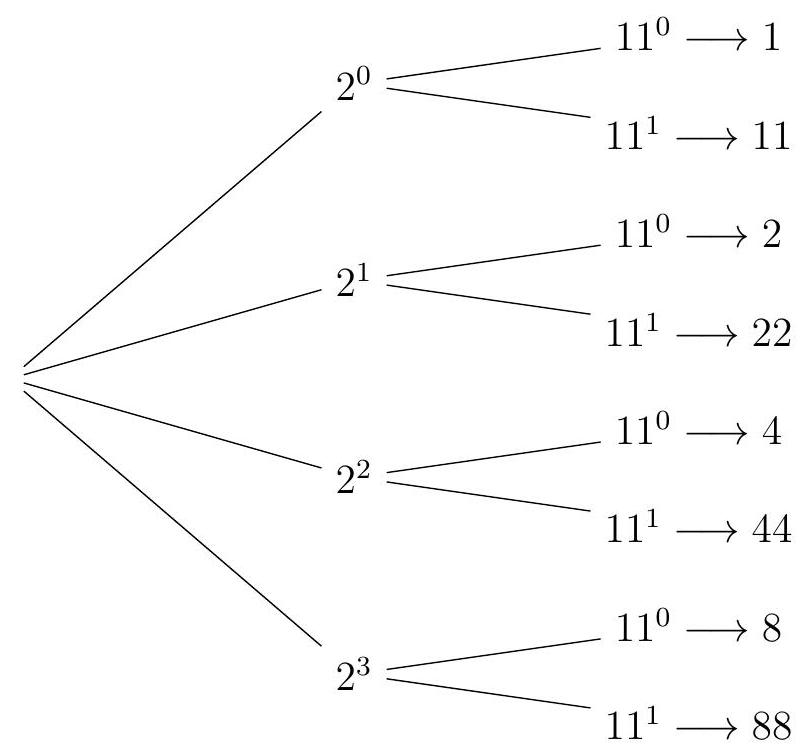
\includegraphics[max width=0.5\linewidth, center]{2025_02_06_9ce8241190b3f203dae3g-5}

Ainsi, les diviseurs de 88 sont $1,2,4,8,11,22,44$ et 88 .
\end{example}

\begin{proposition}{}{}
Soient $n$ et $m$ deux entiers naturels supérieurs ou égaux à 2 . On suppose, quitte à utiliser des exposants nuls, que $m$ et $n$ peuvent s'écrire sous forme de produit de nombres premiers de la manière suivante:

$$
n=p_{1}^{\alpha_{1}} \times p_{2}^{\alpha_{2}} \times \ldots \times p_{k}^{\alpha_{k}} \quad \text { et } \quad m=p_{1}^{\beta_{1}} \times p_{2}^{\beta_{2}} \times \ldots \times p_{k}^{\beta_{k}} .
$$

On a alors :

\begin{itemize}[noitemsep,topsep=0pt]
  \item $\operatorname{PGCD}(n ; m)=p_{1}^{\min \left(\alpha_{1} \beta_{1}\right)} \times p_{2}^{\min \left(\alpha_{2} \beta_{2}\right)} \times \ldots \times p_{k}^{\min \left(\alpha_{k} \beta_{k}\right)}$
  \item $\operatorname{PPCM}(n ; m)=p_{1}^{\max \left(\alpha_{1} \beta_{1}\right)} \times p_{2}^{\max \left(\alpha_{2} \beta_{2}\right)} \times \ldots \times p_{k}^{\max \left(\alpha_{k} \beta_{k}\right)}$
\end{itemize}
\end{proposition}

\begin{example}
Les décompositions de 126 et 196 sont $126=2 \times 3^{2} \times 7$ et $196=2^{2} \times 3^{0} \times 7^{2}$.\\
Par conséquent, $\operatorname{PGCD}(126 ; 196)=2^{1} \times 3^{0} \times 7^{1}=14$.\\
De plus, $\operatorname{PPCM}(126 ; 196)=2^{2} \times 3^{2} \times 7^{2}=1764$.
\end{example}

\begin{remark}
En pratique, pour des grands nombres, la décomposition en produit de nombres premiers est difficile à obtenir. La meilleure méthode pour déterminer un PGCD reste donc l'algorithme d'Euclide. La propriété 6 ci-dessus peut néanmoins avoir un intérêt pour résoudre des questions d'ordre théorique.
\end{remark}

\section{Petit théorème de Fermat}
\begin{proposition}{Lemme}{}
  Si $p$ est un nombre premier et $k$ un entier tel que $1 \leqslant k \leqslant p-1$, alors $p$ divise $\dbinom{p}{k}$.
\end{proposition}
\begin{demo}
Soit $p$ un nombre premier et $k$ un entier tel que $1 \leqslant k \leqslant p-1$. On a $\dbinom{p}{k}=\dfrac{p!}{k!(p-k)!}$.\\
Par conséquent, $k!\dbinom{p}{k}=\dfrac{p!}{(p-k)!}$.\\
Comme $k \geqslant 1$, on voit que $p$ divise $\dfrac{p!}{(p-k)!}$.\\
Cela signifie que $p$ divise $k!\dbinom{p}{k}$.\\
Or, comme $k \leqslant p-1$, $k$ ! et $p$ sont premiers entre eux.\\
D'après le théorème de Gauss, on en déduit donc que $p$ divise $\dbinom{p}{k}$.
\end{demo}

\begin{proposition}{}{}
Si $p$ est un nombre premier alors pour tout entier $a, a^{p} \equiv a[p]$.
\end{proposition}

\begin{demo}
Soit $p$ un nombre premier.\\
Montrons par récurrence que la propriété $\mathcal{P}(a):<a^{p} \equiv a[p] »$ est vraie pour tout entier $a \geqslant 0$.\\
\textbf{Initialisation :} Il est clair que $\mathcal{P}(0)$ est vraie.\\
\textbf{Hérédité :} Supposons que $\mathcal{P}(a)$ soit vraie pour un certain entier $a \geqslant 0$ et montrons qu'alors $\mathcal{P}(a+1)$ est vraie.\\
On a:

$$
\begin{aligned}
(a+1)^{p} & =\sum_{k=0}^{p}\binom{p}{k} a^{k} \\
& =1+\left(\sum_{k=1}^{p-1}\binom{p}{k} a^{k}\right)+a^{p} \\
& \equiv 1+a^{p}[p] \quad\left(\text { car pour tout } 1 \leqslant k \leqslant p-1, p \text { divise }\binom{p}{k}\right) \\
& \equiv 1+a[p] \quad \text { (d'après l'hypothèse } \mathcal{P}(a))
\end{aligned}
$$

Ainsi, on a montré que $(a+1)^{p}=a+1$ donc $\mathcal{P}(a)+1$ est vraie.
\end{demo}

\newpage
\begin{proposition}{Petit théorème de Fermat}{}
Si $p$ est un nombre premier et si $a$ est un entier non divisible par $p$, alors $a^{p-1} \equiv 1[p]$.
\end{proposition}

\begin{remark}
Dans le cas où $a$ est divisible par $p$, on a $a^{p-1} \equiv 0[p]$.
\end{remark}

\begin{demo}
Soit $p$ un nombre premier et $a$ un entier non divisible par $p$.\\
D'après la propriété précédente, $a^{p} \equiv a[p] \quad(\star)$.\\
Or, comme $p$ est premier et ne divise pas $a, p$ est donc premier avec $a$.\\
Par conséquent, $a$ est inversible modulo $p$.\\
En multipliant l'égalité ( $\star$ ) par l'inverse de $a$, on obtient $a^{p-1} \equiv 1[p]$.
\end{demo}

\begin{example}
29 est un nombre premier et 250 n'est pas divisible par 29 . On a donc $250^{28} \equiv 1$ [29].
\end{example}

\noindent
\begin{minipage}{.7\textwidth}
  \begin{history}{Grand théorème de Fermat}{}
    Le petit théorème de Fermat est à distinguer du grand théorème de Fermat, beaucoup plus difficile à démontrer. Ce théorème indique que l'équation $x^{n}+y^{n}=z^{n}$ (où $n$ est un entier supérieur ou égal à 3) admet aucune solution entière et non nulle. Dans un ouvrage publié au XVIIe siècle, Pierre de Fermat avait énoncé ce résultat en ajoutant : «j'en ai découvert une démonstration véritablement merveilleuse que cette marge est trop étroite pour contenir ». Il s'était vraisemblablement trompé et de nombreux mathématiciens ont cherché à démontré ce résultat depuis. En particulier, au XIX ${ }^{e}$ siècle, Sophie Germain (1776-1831) a démontré le théorème pour une certaine classe d'exposants (les nombres premiers dits de Sophie Germain). Finalement, ce n'est qu'en 1994, plus de 350 ans après que Fermat ait énoncé le théorème, que le britannique Andrew Wiles parvient à une démonstration complète.
  \end{history}
\end{minipage}
\hspace{1em}
\begin{minipage}{0.35\textwidth}
  \begin{tcolorbox}[colback=white,colframe=BrownHist]
    \centering
    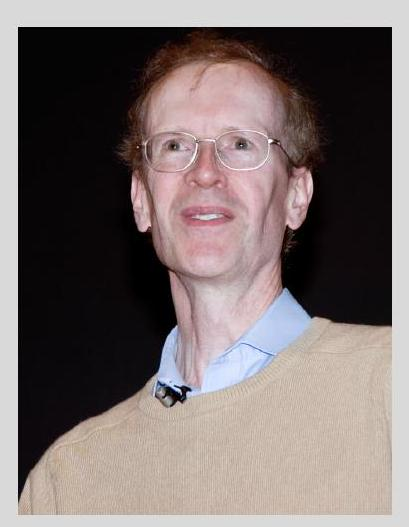
\includegraphics[max width=\textwidth, center]{2025_02_06_9ce8241190b3f203dae3g-7(1)}
    Andrew Wiles
  \end{tcolorbox}
\end{minipage}

\vspace{1em}

\begin{savoir}{}{}
\begin{itemize}[noitemsep,topsep=0pt]
  \item Déterminer si un nombre est premier ou non.
  \item Dresser la liste des nombre premiers inférieurs à un nombre donné.
  \item Décomposer un nombre en produit de facteurs premiers.
  \item Déterminer les diviseurs d'un entier à partir de la décomposition en facteurs premiers.
  \item Déterminer le PGCD et le PPCM de deux entiers à partir de la décomposition en facteurs premiers.
  \item Cacluler des puissances modulo un nombre premier en utilisant le petit théorème de Fermat.
  \item Utiliser un raisonnement par récurrence forte.
\end{itemize}
\end{savoir}

\end{document}